\documentclass[a4paper,12pt]{article}

\usepackage[utf8]{inputenc}
\usepackage{geometry}
\usepackage{graphicx}
\usepackage{amsmath}
\usepackage{hyperref}

\geometry{margin=1in}

\title{Electronics Experiment Preview: Feedback Circuit}
\author{B13901165張勝勛, B13901020陳諺德}
\date{\today}

% Language and font packages
\usepackage{ctex} % Chinese support

% Pseudocode and algorithm packages
% \usepackage{algorithm2e} % Advanced algorithm writing
% \usepackage{algpseudocode} % Pseudocode environment for algorithms

% Fancy style packages
\usepackage{fancyhdr} % Custom headers/footers
\usepackage{color} % Color support
\usepackage{xcolor} % Extended color support
\usepackage{tcolorbox} % Colored boxes
\usepackage{framed} % Framed environments

% Math and symbol packages
\usepackage{amsfonts}
\usepackage{amssymb}
\usepackage{mathtools}

% Table and figure packages
% \usepackage{booktabs} % Professional tables
% \usepackage{multirow} % Multi-row tables
% \usepackage{caption} % Custom captions
\usepackage{subcaption} % Subfigures

% Miscellaneous
\usepackage{enumitem} % Custom lists
\usepackage{listings} % Code listings
\usepackage{tikz} % Drawing diagrams
\usepackage{pgfplots} % For plotting graphs
\usepackage{float}

\begin{document}
\renewcommand{\figurename}{圖}
\maketitle

\section{Experiment setup}
\begin{figure}[H]
    \centering
    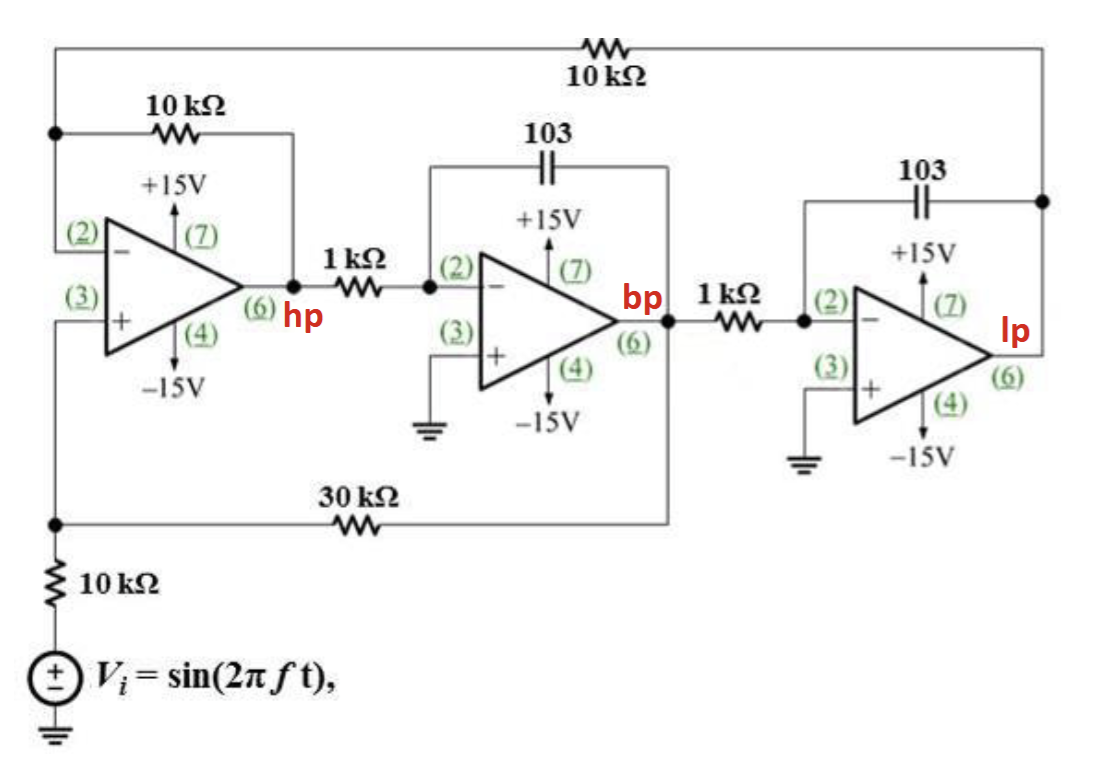
\includegraphics[width=0.8\textwidth]{exp_setup.png}
    \caption{Experiment setup}
    \label{fig:example}
\end{figure}

\section{experiment goals}
\begin{itemize}
    \item find the maximum voltage gain ($A_{max}$) of the feedback circuit.
    \item plot the band-pass amplitude-frequency curve of this circuit
    \item find $f_{L3dB\_BP}$, $f_{H3dB\_BP}$, and $BW$
\end{itemize}

\section{Attention}
\begin{itemize}
    \item input frequency is from 500 Hz to 200 kHz.  
    \item the DC high voltage is 15 V, and the DC low voltage is -15 V.
    \item read the configuration of TL084 and uA741 before the experiment.
\end{itemize}

\end{document}